
% Default to the notebook output style

    


% Inherit from the specified cell style.




    
\documentclass[11pt]{article}

    
    
    \usepackage[T1]{fontenc}
    % Nicer default font (+ math font) than Computer Modern for most use cases
    \usepackage{mathpazo}
	\usepackage{float}
    % Basic figure setup, for now with no caption control since it's done
    % automatically by Pandoc (which extracts ![](path) syntax from Markdown).
    \usepackage{graphicx}
    % We will generate all images so they have a width \maxwidth. This means
    % that they will get their normal width if they fit onto the page, but
    % are scaled down if they would overflow the margins.
    \makeatletter
    \def\maxwidth{\ifdim\Gin@nat@width>\linewidth\linewidth
    \else\Gin@nat@width\fi}
    \makeatother
    \let\Oldincludegraphics\includegraphics
    % Set max figure width to be 80% of text width, for now hardcoded.
    \renewcommand{\includegraphics}[1]{\Oldincludegraphics[width=.8\maxwidth]{#1}}
    % Ensure that by default, figures have no caption (until we provide a
    % proper Figure object with a Caption API and a way to capture that
    % in the conversion process - todo).
    \usepackage{caption}
    \DeclareCaptionLabelFormat{nolabel}{}
    \captionsetup{labelformat=nolabel}

    \usepackage{adjustbox} % Used to constrain images to a maximum size 
    \usepackage{xcolor} % Allow colors to be defined
    \usepackage{enumerate} % Needed for markdown enumerations to work
    \usepackage{geometry} % Used to adjust the document margins
    \usepackage{amsmath} % Equations
    \usepackage{amssymb} % Equations
    \usepackage{textcomp} % defines textquotesingle
    % Hack from http://tex.stackexchange.com/a/47451/13684:
    \AtBeginDocument{%
        \def\PYZsq{\textquotesingle}% Upright quotes in Pygmentized code
    }
    \usepackage{upquote} % Upright quotes for verbatim code
    \usepackage{eurosym} % defines \euro
    \usepackage[mathletters]{ucs} % Extended unicode (utf-8) support
    \usepackage[utf8x]{inputenc} % Allow utf-8 characters in the tex document
    \usepackage{fancyvrb} % verbatim replacement that allows latex
    \usepackage{grffile} % extends the file name processing of package graphics 
                         % to support a larger range 
    % The hyperref package gives us a pdf with properly built
    % internal navigation ('pdf bookmarks' for the table of contents,
    % internal cross-reference links, web links for URLs, etc.)
    \usepackage{hyperref}
    \usepackage{longtable} % longtable support required by pandoc >1.10
    \usepackage{booktabs}  % table support for pandoc > 1.12.2
    \usepackage[inline]{enumitem} % IRkernel/repr support (it uses the enumerate* environment)
    \usepackage[normalem]{ulem} % ulem is needed to support strikethroughs (\sout)
                                % normalem makes italics be italics, not underlines
    

    
    
    % Colors for the hyperref package
    \definecolor{urlcolor}{rgb}{0,.145,.698}
    \definecolor{linkcolor}{rgb}{.71,0.21,0.01}
    \definecolor{citecolor}{rgb}{.12,.54,.11}

    % ANSI colors
    \definecolor{ansi-black}{HTML}{3E424D}
    \definecolor{ansi-black-intense}{HTML}{282C36}
    \definecolor{ansi-red}{HTML}{E75C58}
    \definecolor{ansi-red-intense}{HTML}{B22B31}
    \definecolor{ansi-green}{HTML}{00A250}
    \definecolor{ansi-green-intense}{HTML}{007427}
    \definecolor{ansi-yellow}{HTML}{DDB62B}
    \definecolor{ansi-yellow-intense}{HTML}{B27D12}
    \definecolor{ansi-blue}{HTML}{208FFB}
    \definecolor{ansi-blue-intense}{HTML}{0065CA}
    \definecolor{ansi-magenta}{HTML}{D160C4}
    \definecolor{ansi-magenta-intense}{HTML}{A03196}
    \definecolor{ansi-cyan}{HTML}{60C6C8}
    \definecolor{ansi-cyan-intense}{HTML}{258F8F}
    \definecolor{ansi-white}{HTML}{C5C1B4}
    \definecolor{ansi-white-intense}{HTML}{A1A6B2}

    % commands and environments needed by pandoc snippets
    % extracted from the output of `pandoc -s`
    \providecommand{\tightlist}{%
      \setlength{\itemsep}{0pt}\setlength{\parskip}{0pt}}
    \DefineVerbatimEnvironment{Highlighting}{Verbatim}{commandchars=\\\{\}}
    % Add ',fontsize=\small' for more characters per line
    \newenvironment{Shaded}{}{}
    \newcommand{\KeywordTok}[1]{\textcolor[rgb]{0.00,0.44,0.13}{\textbf{{#1}}}}
    \newcommand{\DataTypeTok}[1]{\textcolor[rgb]{0.56,0.13,0.00}{{#1}}}
    \newcommand{\DecValTok}[1]{\textcolor[rgb]{0.25,0.63,0.44}{{#1}}}
    \newcommand{\BaseNTok}[1]{\textcolor[rgb]{0.25,0.63,0.44}{{#1}}}
    \newcommand{\FloatTok}[1]{\textcolor[rgb]{0.25,0.63,0.44}{{#1}}}
    \newcommand{\CharTok}[1]{\textcolor[rgb]{0.25,0.44,0.63}{{#1}}}
    \newcommand{\StringTok}[1]{\textcolor[rgb]{0.25,0.44,0.63}{{#1}}}
    \newcommand{\CommentTok}[1]{\textcolor[rgb]{0.38,0.63,0.69}{\textit{{#1}}}}
    \newcommand{\OtherTok}[1]{\textcolor[rgb]{0.00,0.44,0.13}{{#1}}}
    \newcommand{\AlertTok}[1]{\textcolor[rgb]{1.00,0.00,0.00}{\textbf{{#1}}}}
    \newcommand{\FunctionTok}[1]{\textcolor[rgb]{0.02,0.16,0.49}{{#1}}}
    \newcommand{\RegionMarkerTok}[1]{{#1}}
    \newcommand{\ErrorTok}[1]{\textcolor[rgb]{1.00,0.00,0.00}{\textbf{{#1}}}}
    \newcommand{\NormalTok}[1]{{#1}}
    
    % Additional commands for more recent versions of Pandoc
    \newcommand{\ConstantTok}[1]{\textcolor[rgb]{0.53,0.00,0.00}{{#1}}}
    \newcommand{\SpecialCharTok}[1]{\textcolor[rgb]{0.25,0.44,0.63}{{#1}}}
    \newcommand{\VerbatimStringTok}[1]{\textcolor[rgb]{0.25,0.44,0.63}{{#1}}}
    \newcommand{\SpecialStringTok}[1]{\textcolor[rgb]{0.73,0.40,0.53}{{#1}}}
    \newcommand{\ImportTok}[1]{{#1}}
    \newcommand{\DocumentationTok}[1]{\textcolor[rgb]{0.73,0.13,0.13}{\textit{{#1}}}}
    \newcommand{\AnnotationTok}[1]{\textcolor[rgb]{0.38,0.63,0.69}{\textbf{\textit{{#1}}}}}
    \newcommand{\CommentVarTok}[1]{\textcolor[rgb]{0.38,0.63,0.69}{\textbf{\textit{{#1}}}}}
    \newcommand{\VariableTok}[1]{\textcolor[rgb]{0.10,0.09,0.49}{{#1}}}
    \newcommand{\ControlFlowTok}[1]{\textcolor[rgb]{0.00,0.44,0.13}{\textbf{{#1}}}}
    \newcommand{\OperatorTok}[1]{\textcolor[rgb]{0.40,0.40,0.40}{{#1}}}
    \newcommand{\BuiltInTok}[1]{{#1}}
    \newcommand{\ExtensionTok}[1]{{#1}}
    \newcommand{\PreprocessorTok}[1]{\textcolor[rgb]{0.74,0.48,0.00}{{#1}}}
    \newcommand{\AttributeTok}[1]{\textcolor[rgb]{0.49,0.56,0.16}{{#1}}}
    \newcommand{\InformationTok}[1]{\textcolor[rgb]{0.38,0.63,0.69}{\textbf{\textit{{#1}}}}}
    \newcommand{\WarningTok}[1]{\textcolor[rgb]{0.38,0.63,0.69}{\textbf{\textit{{#1}}}}}
    
    
    % Define a nice break command that doesn't care if a line doesn't already
    % exist.
    \def\br{\hspace*{\fill} \\* }
    % Math Jax compatability definitions
    \def\gt{>}
    \def\lt{<}
    % Document parameters
    \title{CMM201 Week 4}
    
    
    

    % Pygments definitions
    
\makeatletter
\def\PY@reset{\let\PY@it=\relax \let\PY@bf=\relax%
    \let\PY@ul=\relax \let\PY@tc=\relax%
    \let\PY@bc=\relax \let\PY@ff=\relax}
\def\PY@tok#1{\csname PY@tok@#1\endcsname}
\def\PY@toks#1+{\ifx\relax#1\empty\else%
    \PY@tok{#1}\expandafter\PY@toks\fi}
\def\PY@do#1{\PY@bc{\PY@tc{\PY@ul{%
    \PY@it{\PY@bf{\PY@ff{#1}}}}}}}
\def\PY#1#2{\PY@reset\PY@toks#1+\relax+\PY@do{#2}}

\expandafter\def\csname PY@tok@w\endcsname{\def\PY@tc##1{\textcolor[rgb]{0.73,0.73,0.73}{##1}}}
\expandafter\def\csname PY@tok@c\endcsname{\let\PY@it=\textit\def\PY@tc##1{\textcolor[rgb]{0.25,0.50,0.50}{##1}}}
\expandafter\def\csname PY@tok@cp\endcsname{\def\PY@tc##1{\textcolor[rgb]{0.74,0.48,0.00}{##1}}}
\expandafter\def\csname PY@tok@k\endcsname{\let\PY@bf=\textbf\def\PY@tc##1{\textcolor[rgb]{0.00,0.50,0.00}{##1}}}
\expandafter\def\csname PY@tok@kp\endcsname{\def\PY@tc##1{\textcolor[rgb]{0.00,0.50,0.00}{##1}}}
\expandafter\def\csname PY@tok@kt\endcsname{\def\PY@tc##1{\textcolor[rgb]{0.69,0.00,0.25}{##1}}}
\expandafter\def\csname PY@tok@o\endcsname{\def\PY@tc##1{\textcolor[rgb]{0.40,0.40,0.40}{##1}}}
\expandafter\def\csname PY@tok@ow\endcsname{\let\PY@bf=\textbf\def\PY@tc##1{\textcolor[rgb]{0.67,0.13,1.00}{##1}}}
\expandafter\def\csname PY@tok@nb\endcsname{\def\PY@tc##1{\textcolor[rgb]{0.00,0.50,0.00}{##1}}}
\expandafter\def\csname PY@tok@nf\endcsname{\def\PY@tc##1{\textcolor[rgb]{0.00,0.00,1.00}{##1}}}
\expandafter\def\csname PY@tok@nc\endcsname{\let\PY@bf=\textbf\def\PY@tc##1{\textcolor[rgb]{0.00,0.00,1.00}{##1}}}
\expandafter\def\csname PY@tok@nn\endcsname{\let\PY@bf=\textbf\def\PY@tc##1{\textcolor[rgb]{0.00,0.00,1.00}{##1}}}
\expandafter\def\csname PY@tok@ne\endcsname{\let\PY@bf=\textbf\def\PY@tc##1{\textcolor[rgb]{0.82,0.25,0.23}{##1}}}
\expandafter\def\csname PY@tok@nv\endcsname{\def\PY@tc##1{\textcolor[rgb]{0.10,0.09,0.49}{##1}}}
\expandafter\def\csname PY@tok@no\endcsname{\def\PY@tc##1{\textcolor[rgb]{0.53,0.00,0.00}{##1}}}
\expandafter\def\csname PY@tok@nl\endcsname{\def\PY@tc##1{\textcolor[rgb]{0.63,0.63,0.00}{##1}}}
\expandafter\def\csname PY@tok@ni\endcsname{\let\PY@bf=\textbf\def\PY@tc##1{\textcolor[rgb]{0.60,0.60,0.60}{##1}}}
\expandafter\def\csname PY@tok@na\endcsname{\def\PY@tc##1{\textcolor[rgb]{0.49,0.56,0.16}{##1}}}
\expandafter\def\csname PY@tok@nt\endcsname{\let\PY@bf=\textbf\def\PY@tc##1{\textcolor[rgb]{0.00,0.50,0.00}{##1}}}
\expandafter\def\csname PY@tok@nd\endcsname{\def\PY@tc##1{\textcolor[rgb]{0.67,0.13,1.00}{##1}}}
\expandafter\def\csname PY@tok@s\endcsname{\def\PY@tc##1{\textcolor[rgb]{0.73,0.13,0.13}{##1}}}
\expandafter\def\csname PY@tok@sd\endcsname{\let\PY@it=\textit\def\PY@tc##1{\textcolor[rgb]{0.73,0.13,0.13}{##1}}}
\expandafter\def\csname PY@tok@si\endcsname{\let\PY@bf=\textbf\def\PY@tc##1{\textcolor[rgb]{0.73,0.40,0.53}{##1}}}
\expandafter\def\csname PY@tok@se\endcsname{\let\PY@bf=\textbf\def\PY@tc##1{\textcolor[rgb]{0.73,0.40,0.13}{##1}}}
\expandafter\def\csname PY@tok@sr\endcsname{\def\PY@tc##1{\textcolor[rgb]{0.73,0.40,0.53}{##1}}}
\expandafter\def\csname PY@tok@ss\endcsname{\def\PY@tc##1{\textcolor[rgb]{0.10,0.09,0.49}{##1}}}
\expandafter\def\csname PY@tok@sx\endcsname{\def\PY@tc##1{\textcolor[rgb]{0.00,0.50,0.00}{##1}}}
\expandafter\def\csname PY@tok@m\endcsname{\def\PY@tc##1{\textcolor[rgb]{0.40,0.40,0.40}{##1}}}
\expandafter\def\csname PY@tok@gh\endcsname{\let\PY@bf=\textbf\def\PY@tc##1{\textcolor[rgb]{0.00,0.00,0.50}{##1}}}
\expandafter\def\csname PY@tok@gu\endcsname{\let\PY@bf=\textbf\def\PY@tc##1{\textcolor[rgb]{0.50,0.00,0.50}{##1}}}
\expandafter\def\csname PY@tok@gd\endcsname{\def\PY@tc##1{\textcolor[rgb]{0.63,0.00,0.00}{##1}}}
\expandafter\def\csname PY@tok@gi\endcsname{\def\PY@tc##1{\textcolor[rgb]{0.00,0.63,0.00}{##1}}}
\expandafter\def\csname PY@tok@gr\endcsname{\def\PY@tc##1{\textcolor[rgb]{1.00,0.00,0.00}{##1}}}
\expandafter\def\csname PY@tok@ge\endcsname{\let\PY@it=\textit}
\expandafter\def\csname PY@tok@gs\endcsname{\let\PY@bf=\textbf}
\expandafter\def\csname PY@tok@gp\endcsname{\let\PY@bf=\textbf\def\PY@tc##1{\textcolor[rgb]{0.00,0.00,0.50}{##1}}}
\expandafter\def\csname PY@tok@go\endcsname{\def\PY@tc##1{\textcolor[rgb]{0.53,0.53,0.53}{##1}}}
\expandafter\def\csname PY@tok@gt\endcsname{\def\PY@tc##1{\textcolor[rgb]{0.00,0.27,0.87}{##1}}}
\expandafter\def\csname PY@tok@err\endcsname{\def\PY@bc##1{\setlength{\fboxsep}{0pt}\fcolorbox[rgb]{1.00,0.00,0.00}{1,1,1}{\strut ##1}}}
\expandafter\def\csname PY@tok@kc\endcsname{\let\PY@bf=\textbf\def\PY@tc##1{\textcolor[rgb]{0.00,0.50,0.00}{##1}}}
\expandafter\def\csname PY@tok@kd\endcsname{\let\PY@bf=\textbf\def\PY@tc##1{\textcolor[rgb]{0.00,0.50,0.00}{##1}}}
\expandafter\def\csname PY@tok@kn\endcsname{\let\PY@bf=\textbf\def\PY@tc##1{\textcolor[rgb]{0.00,0.50,0.00}{##1}}}
\expandafter\def\csname PY@tok@kr\endcsname{\let\PY@bf=\textbf\def\PY@tc##1{\textcolor[rgb]{0.00,0.50,0.00}{##1}}}
\expandafter\def\csname PY@tok@bp\endcsname{\def\PY@tc##1{\textcolor[rgb]{0.00,0.50,0.00}{##1}}}
\expandafter\def\csname PY@tok@fm\endcsname{\def\PY@tc##1{\textcolor[rgb]{0.00,0.00,1.00}{##1}}}
\expandafter\def\csname PY@tok@vc\endcsname{\def\PY@tc##1{\textcolor[rgb]{0.10,0.09,0.49}{##1}}}
\expandafter\def\csname PY@tok@vg\endcsname{\def\PY@tc##1{\textcolor[rgb]{0.10,0.09,0.49}{##1}}}
\expandafter\def\csname PY@tok@vi\endcsname{\def\PY@tc##1{\textcolor[rgb]{0.10,0.09,0.49}{##1}}}
\expandafter\def\csname PY@tok@vm\endcsname{\def\PY@tc##1{\textcolor[rgb]{0.10,0.09,0.49}{##1}}}
\expandafter\def\csname PY@tok@sa\endcsname{\def\PY@tc##1{\textcolor[rgb]{0.73,0.13,0.13}{##1}}}
\expandafter\def\csname PY@tok@sb\endcsname{\def\PY@tc##1{\textcolor[rgb]{0.73,0.13,0.13}{##1}}}
\expandafter\def\csname PY@tok@sc\endcsname{\def\PY@tc##1{\textcolor[rgb]{0.73,0.13,0.13}{##1}}}
\expandafter\def\csname PY@tok@dl\endcsname{\def\PY@tc##1{\textcolor[rgb]{0.73,0.13,0.13}{##1}}}
\expandafter\def\csname PY@tok@s2\endcsname{\def\PY@tc##1{\textcolor[rgb]{0.73,0.13,0.13}{##1}}}
\expandafter\def\csname PY@tok@sh\endcsname{\def\PY@tc##1{\textcolor[rgb]{0.73,0.13,0.13}{##1}}}
\expandafter\def\csname PY@tok@s1\endcsname{\def\PY@tc##1{\textcolor[rgb]{0.73,0.13,0.13}{##1}}}
\expandafter\def\csname PY@tok@mb\endcsname{\def\PY@tc##1{\textcolor[rgb]{0.40,0.40,0.40}{##1}}}
\expandafter\def\csname PY@tok@mf\endcsname{\def\PY@tc##1{\textcolor[rgb]{0.40,0.40,0.40}{##1}}}
\expandafter\def\csname PY@tok@mh\endcsname{\def\PY@tc##1{\textcolor[rgb]{0.40,0.40,0.40}{##1}}}
\expandafter\def\csname PY@tok@mi\endcsname{\def\PY@tc##1{\textcolor[rgb]{0.40,0.40,0.40}{##1}}}
\expandafter\def\csname PY@tok@il\endcsname{\def\PY@tc##1{\textcolor[rgb]{0.40,0.40,0.40}{##1}}}
\expandafter\def\csname PY@tok@mo\endcsname{\def\PY@tc##1{\textcolor[rgb]{0.40,0.40,0.40}{##1}}}
\expandafter\def\csname PY@tok@ch\endcsname{\let\PY@it=\textit\def\PY@tc##1{\textcolor[rgb]{0.25,0.50,0.50}{##1}}}
\expandafter\def\csname PY@tok@cm\endcsname{\let\PY@it=\textit\def\PY@tc##1{\textcolor[rgb]{0.25,0.50,0.50}{##1}}}
\expandafter\def\csname PY@tok@cpf\endcsname{\let\PY@it=\textit\def\PY@tc##1{\textcolor[rgb]{0.25,0.50,0.50}{##1}}}
\expandafter\def\csname PY@tok@c1\endcsname{\let\PY@it=\textit\def\PY@tc##1{\textcolor[rgb]{0.25,0.50,0.50}{##1}}}
\expandafter\def\csname PY@tok@cs\endcsname{\let\PY@it=\textit\def\PY@tc##1{\textcolor[rgb]{0.25,0.50,0.50}{##1}}}

\def\PYZbs{\char`\\}
\def\PYZus{\char`\_}
\def\PYZob{\char`\{}
\def\PYZcb{\char`\}}
\def\PYZca{\char`\^}
\def\PYZam{\char`\&}
\def\PYZlt{\char`\<}
\def\PYZgt{\char`\>}
\def\PYZsh{\char`\#}
\def\PYZpc{\char`\%}
\def\PYZdl{\char`\$}
\def\PYZhy{\char`\-}
\def\PYZsq{\char`\'}
\def\PYZdq{\char`\"}
\def\PYZti{\char`\~}
% for compatibility with earlier versions
\def\PYZat{@}
\def\PYZlb{[}
\def\PYZrb{]}
\makeatother


    % Exact colors from NB
    \definecolor{incolor}{rgb}{0.0, 0.0, 0.5}
    \definecolor{outcolor}{rgb}{0.545, 0.0, 0.0}



    
    % Prevent overflowing lines due to hard-to-break entities
    \sloppy 
    % Setup hyperref package
    \hypersetup{
      breaklinks=true,  % so long urls are correctly broken across lines
      colorlinks=true,
      urlcolor=urlcolor,
      linkcolor=linkcolor,
      citecolor=citecolor,
      }
    % Slightly bigger margins than the latex defaults
    
    \geometry{verbose,tmargin=1in,bmargin=1in,lmargin=1in,rmargin=1in}
    
    
	\date{}
    \begin{document}
    
    
    \maketitle
    
   


    \hypertarget{conditional-statements-in-python}{%
\section{CONDITIONAL STATEMENTS IN
PYTHON}\label{conditional-statements-in-python}}

    \hypertarget{aims-of-the-lecture}{%
\subsection{Aims of the Lecture}\label{aims-of-the-lecture}}

\begin{itemize}
\tightlist
\item
  Learn and understand the different conditional statements contained in
  Python.
\item
  Exemplify practical uses of each statement.
\item
  Learn how data types and data structures interact with these
  conditional statements
\end{itemize}

    \hypertarget{additional-reading-and-sources}{%
\subsection{Additional Reading and
Sources}\label{additional-reading-and-sources}}

\begin{itemize}
\tightlist
\item
  \href{https://www.w3schools.com/python/python_for_loops.asp}{w3schools}
\item
  \href{https://realpython.com/python-conditional-statements/}{Real
  Python}
\end{itemize}

    \hypertarget{the-ifelifelse-conditional-statement}{%
\section{The IF/ELIF/ELSE Conditional
Statement}\label{the-ifelifelse-conditional-statement}}

    \begin{itemize}
\tightlist
\item
  In its most basic form, an \emph{if} statement establishes a condition
  which, if met, executes the statement.
\item
  We use colon (:) to finish the if condition(s).
\item
  Then, we establish the statement using TAB/INDENT.
\end{itemize}

    \begin{Verbatim}[commandchars=\\\{\}]
{\color{incolor}In [{\color{incolor} }]:} \PY{c+c1}{\PYZsh{} example of an if statement}
        \PY{k}{if} \PY{l+m+mi}{1}\PY{o}{\PYZlt{}}\PY{l+m+mi}{2}\PY{p}{:}
            \PY{n+nb}{print}\PY{p}{(}\PY{l+s+s1}{\PYZsq{}}\PY{l+s+s1}{True!}\PY{l+s+s1}{\PYZsq{}}\PY{p}{)}
\end{Verbatim}


    \begin{Verbatim}[commandchars=\\\{\}]
{\color{incolor}In [{\color{incolor} }]:} \PY{c+c1}{\PYZsh{} example of an if statement with two conditions}
        \PY{k}{if} \PY{l+m+mi}{1}\PY{o}{\PYZlt{}}\PY{l+m+mi}{2} \PY{o+ow}{and} \PY{l+s+s1}{\PYZsq{}}\PY{l+s+s1}{P}\PY{l+s+s1}{\PYZsq{}} \PY{o+ow}{in} \PY{l+s+s1}{\PYZsq{}}\PY{l+s+s1}{Python}\PY{l+s+s1}{\PYZsq{}}\PY{p}{:}
            \PY{n+nb}{print}\PY{p}{(}\PY{l+s+s1}{\PYZsq{}}\PY{l+s+s1}{Also true!}\PY{l+s+s1}{\PYZsq{}}\PY{p}{)}
\end{Verbatim}


    \begin{itemize}
\tightlist
\item
  Python is all about indentation (off-side rule).

  \begin{itemize}
  \tightlist
  \item
    Coined after football!
  \end{itemize}
\item
  You need to be careful regarding how statements work!
\end{itemize}

    \begin{itemize}
\tightlist
\item
  This is how Python does it. 
\end{itemize}

\begin{figure}[H]
  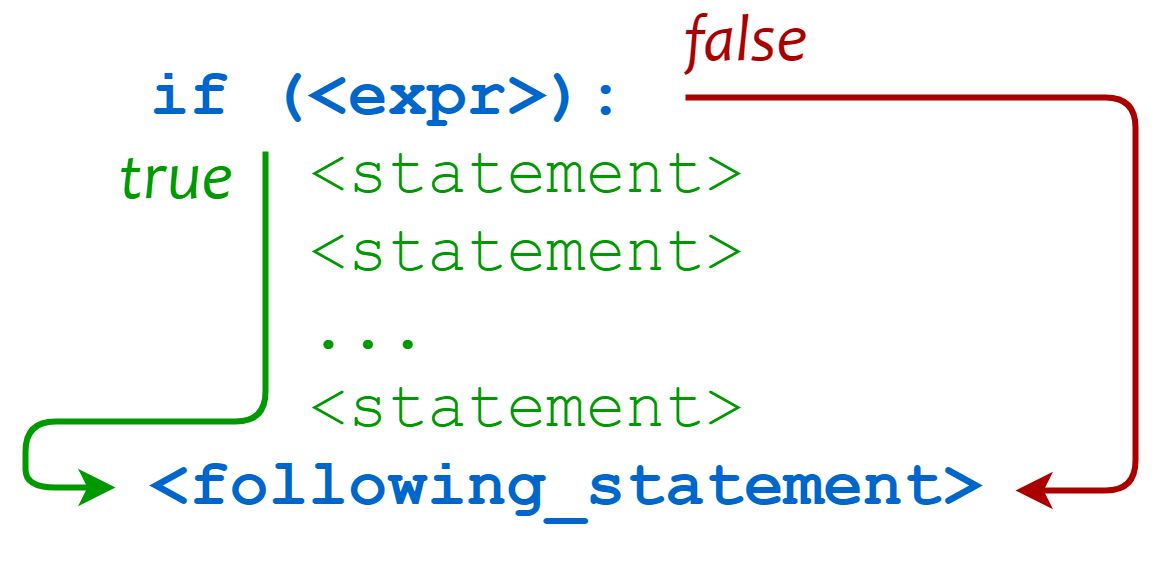
\includegraphics{figs/ifpython.png}
\end{figure}

    \begin{itemize}
\tightlist
\item
  This is how other languages (i.e.~C++/Java/Perl) do it.
\end{itemize}

\begin{figure}[H]
  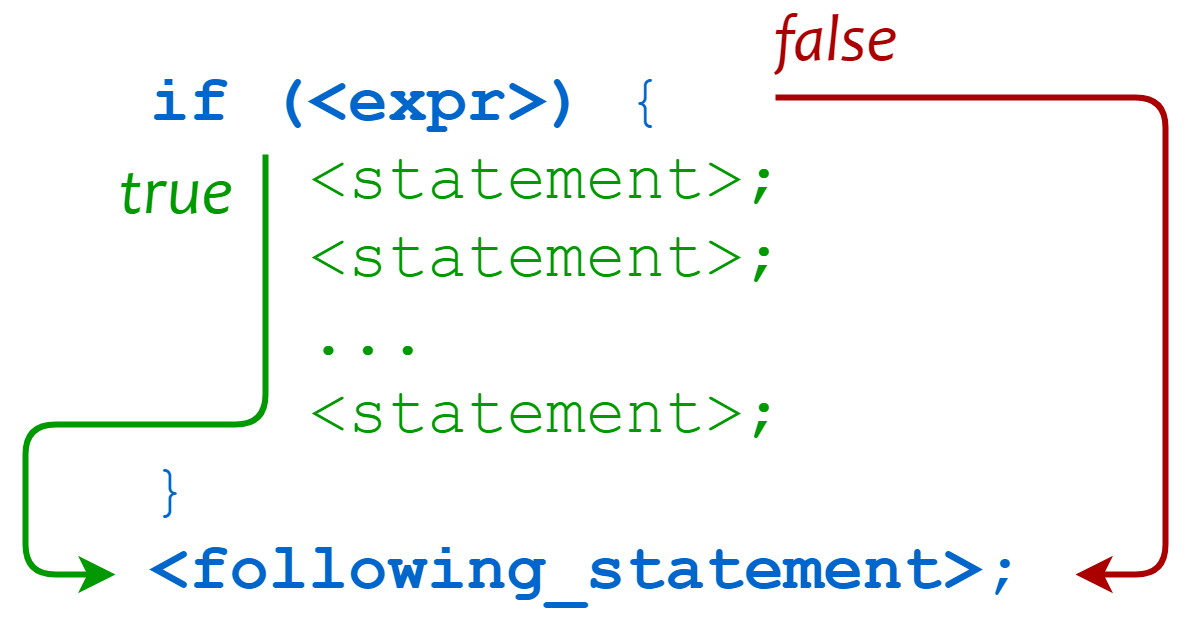
\includegraphics{figs/ifothers.png}
\end{figure}

    \begin{Verbatim}[commandchars=\\\{\}]
{\color{incolor}In [{\color{incolor} }]:} \PY{c+c1}{\PYZsh{} Example}
        \PY{k}{if} \PY{l+m+mi}{3}\PY{o}{\PYZgt{}}\PY{l+m+mi}{2}\PY{p}{:}
            \PY{n+nb}{print}\PY{p}{(}\PY{l+s+s1}{\PYZsq{}}\PY{l+s+s1}{This gets done...}\PY{l+s+s1}{\PYZsq{}}\PY{p}{)}
            \PY{n+nb}{print}\PY{p}{(}\PY{l+s+s1}{\PYZsq{}}\PY{l+s+s1}{...this also gets done...}\PY{l+s+s1}{\PYZsq{}}\PY{p}{)}
        \PY{n+nb}{print}\PY{p}{(}\PY{l+s+s1}{\PYZsq{}}\PY{l+s+s1}{...and this too!}\PY{l+s+s1}{\PYZsq{}}\PY{p}{)}
\end{Verbatim}


    \begin{Verbatim}[commandchars=\\\{\}]
{\color{incolor}In [{\color{incolor} }]:} \PY{c+c1}{\PYZsh{} Example (inverted)}
        \PY{k}{if} \PY{l+m+mi}{3}\PY{o}{\PYZlt{}}\PY{l+m+mi}{2}\PY{p}{:}
            \PY{n+nb}{print}\PY{p}{(}\PY{l+s+s1}{\PYZsq{}}\PY{l+s+s1}{This gets done...}\PY{l+s+s1}{\PYZsq{}}\PY{p}{)}
            \PY{n+nb}{print}\PY{p}{(}\PY{l+s+s1}{\PYZsq{}}\PY{l+s+s1}{...this also gets done...}\PY{l+s+s1}{\PYZsq{}}\PY{p}{)}
        \PY{n+nb}{print}\PY{p}{(}\PY{l+s+s1}{\PYZsq{}}\PY{l+s+s1}{...and this too!}\PY{l+s+s1}{\PYZsq{}}\PY{p}{)}
\end{Verbatim}


    \begin{Verbatim}[commandchars=\\\{\}]
{\color{incolor}In [{\color{incolor} }]:} \PY{c+c1}{\PYZsh{} Does line execute?                        Yes    No}
        \PY{c+c1}{\PYZsh{}                                           \PYZhy{}\PYZhy{}\PYZhy{}    \PYZhy{}\PYZhy{}}
        \PY{k}{if} \PY{l+s+s1}{\PYZsq{}}\PY{l+s+s1}{a}\PY{l+s+s1}{\PYZsq{}} \PY{o+ow}{in} \PY{p}{[}\PY{l+s+s1}{\PYZsq{}}\PY{l+s+s1}{a}\PY{l+s+s1}{\PYZsq{}}\PY{p}{,} \PY{l+m+mf}{3.4}\PY{p}{,} \PY{k+kc}{True}\PY{p}{]}\PY{p}{:}               \PY{c+c1}{\PYZsh{}  x}
            \PY{n+nb}{print}\PY{p}{(}\PY{l+s+s1}{\PYZsq{}}\PY{l+s+s1}{Outer condition is true}\PY{l+s+s1}{\PYZsq{}}\PY{p}{)}      \PY{c+c1}{\PYZsh{}  x}
        
            \PY{k}{if} \PY{l+m+mi}{10} \PY{o}{\PYZgt{}} \PY{l+m+mi}{20}\PY{p}{:}                           \PY{c+c1}{\PYZsh{}  x}
                \PY{n+nb}{print}\PY{p}{(}\PY{l+s+s1}{\PYZsq{}}\PY{l+s+s1}{Inner condition 1}\PY{l+s+s1}{\PYZsq{}}\PY{p}{)}        \PY{c+c1}{\PYZsh{}        x}
        
            \PY{n+nb}{print}\PY{p}{(}\PY{l+s+s1}{\PYZsq{}}\PY{l+s+s1}{Between inner conditions}\PY{l+s+s1}{\PYZsq{}}\PY{p}{)}     \PY{c+c1}{\PYZsh{}  x}
        
            \PY{k}{if} \PY{l+m+mi}{10} \PY{o}{\PYZlt{}} \PY{l+m+mi}{20}\PY{p}{:}                           \PY{c+c1}{\PYZsh{}  x}
                \PY{n+nb}{print}\PY{p}{(}\PY{l+s+s1}{\PYZsq{}}\PY{l+s+s1}{Inner condition 2}\PY{l+s+s1}{\PYZsq{}}\PY{p}{)}        \PY{c+c1}{\PYZsh{}  x}
        
            \PY{n+nb}{print}\PY{p}{(}\PY{l+s+s1}{\PYZsq{}}\PY{l+s+s1}{End of outer condition}\PY{l+s+s1}{\PYZsq{}}\PY{p}{)}       \PY{c+c1}{\PYZsh{}  x}
        \PY{n+nb}{print}\PY{p}{(}\PY{l+s+s1}{\PYZsq{}}\PY{l+s+s1}{After outer condition}\PY{l+s+s1}{\PYZsq{}}\PY{p}{)}            \PY{c+c1}{\PYZsh{}  x}
\end{Verbatim}


    \begin{itemize}
\tightlist
\item
  If you want to test a condition, but after being false test another
  one, use \emph{elif}.
\item
  This has to go aligned with the \emph{if}.
\end{itemize}

    \begin{Verbatim}[commandchars=\\\{\}]
{\color{incolor}In [{\color{incolor} }]:} \PY{k}{if} \PY{l+m+mi}{10}\PY{o}{\PYZgt{}}\PY{l+m+mi}{20}\PY{p}{:}
            \PY{n+nb}{print}\PY{p}{(}\PY{l+s+s1}{\PYZsq{}}\PY{l+s+s1}{nope}\PY{l+s+s1}{\PYZsq{}}\PY{p}{)}
        \PY{k}{elif} \PY{l+m+mi}{10}\PY{o}{\PYZlt{}}\PY{l+m+mi}{20}\PY{p}{:}
            \PY{n+nb}{print}\PY{p}{(}\PY{l+s+s1}{\PYZsq{}}\PY{l+s+s1}{yep}\PY{l+s+s1}{\PYZsq{}}\PY{p}{)}
\end{Verbatim}


    \begin{itemize}
\tightlist
\item
  If the conditions are not met, then we use \emph{else}.
\end{itemize}

    \begin{Verbatim}[commandchars=\\\{\}]
{\color{incolor}In [{\color{incolor} }]:} \PY{k}{if} \PY{l+m+mi}{3}\PY{o}{\PYZlt{}}\PY{l+m+mi}{2}\PY{p}{:}
            \PY{n+nb}{print}\PY{p}{(}\PY{l+s+s1}{\PYZsq{}}\PY{l+s+s1}{Unreal!}\PY{l+s+s1}{\PYZsq{}}\PY{p}{)}
        \PY{k}{else}\PY{p}{:}
            \PY{n+nb}{print}\PY{p}{(}\PY{l+s+s1}{\PYZsq{}}\PY{l+s+s1}{This is the case}\PY{l+s+s1}{\PYZsq{}}\PY{p}{)}
\end{Verbatim}


    \hypertarget{one-line-conditional-statements-and-expressions}{%
\subsection{One-line Conditional Statements and
Expressions}\label{one-line-conditional-statements-and-expressions}}

\begin{itemize}
\tightlist
\item
  Python allows to write conditional statements in one line of code.
\item
  It does not make any difference in computational terms.
\item
  Some people find it more practical.
\end{itemize}

    \begin{Verbatim}[commandchars=\\\{\}]
{\color{incolor}In [{\color{incolor} }]:} \PY{k}{if} \PY{l+m+mi}{1}\PY{o}{\PYZgt{}}\PY{l+m+mi}{0}\PY{p}{:} \PY{n+nb}{print}\PY{p}{(}\PY{l+s+s1}{\PYZsq{}}\PY{l+s+s1}{Yes}\PY{l+s+s1}{\PYZsq{}}\PY{p}{)}\PY{p}{;} \PY{n+nb}{print}\PY{p}{(}\PY{l+s+s1}{\PYZsq{}}\PY{l+s+s1}{sure}\PY{l+s+s1}{\PYZsq{}}\PY{p}{)}
\end{Verbatim}


    \begin{itemize}
\tightlist
\item
  Multiple statements can also be written.
\end{itemize}

    \begin{Verbatim}[commandchars=\\\{\}]
{\color{incolor}In [{\color{incolor} }]:} \PY{n}{x} \PY{o}{=} \PY{l+m+mi}{2}
        \PY{k}{if} \PY{n}{x} \PY{o}{==} \PY{l+m+mi}{1}\PY{p}{:} \PY{n+nb}{print}\PY{p}{(}\PY{l+s+s1}{\PYZsq{}}\PY{l+s+s1}{a}\PY{l+s+s1}{\PYZsq{}}\PY{p}{)}\PY{p}{;} \PY{n+nb}{print}\PY{p}{(}\PY{l+s+s1}{\PYZsq{}}\PY{l+s+s1}{b}\PY{l+s+s1}{\PYZsq{}}\PY{p}{)}\PY{p}{;} \PY{n+nb}{print}\PY{p}{(}\PY{l+s+s1}{\PYZsq{}}\PY{l+s+s1}{c}\PY{l+s+s1}{\PYZsq{}}\PY{p}{)}
        \PY{k}{elif} \PY{n}{x} \PY{o}{==} \PY{l+m+mi}{2}\PY{p}{:} \PY{n+nb}{print}\PY{p}{(}\PY{l+s+s1}{\PYZsq{}}\PY{l+s+s1}{d}\PY{l+s+s1}{\PYZsq{}}\PY{p}{)}\PY{p}{;} \PY{n+nb}{print}\PY{p}{(}\PY{l+s+s1}{\PYZsq{}}\PY{l+s+s1}{e}\PY{l+s+s1}{\PYZsq{}}\PY{p}{)}
        \PY{k}{else}\PY{p}{:} \PY{n+nb}{print}\PY{p}{(}\PY{l+s+s1}{\PYZsq{}}\PY{l+s+s1}{f}\PY{l+s+s1}{\PYZsq{}}\PY{p}{)}\PY{p}{;} \PY{n+nb}{print}\PY{p}{(}\PY{l+s+s1}{\PYZsq{}}\PY{l+s+s1}{g}\PY{l+s+s1}{\PYZsq{}}\PY{p}{)}
\end{Verbatim}


    \begin{itemize}
\tightlist
\item
  Conditional (or ternary) operations are also supported in Python.
\item
  This has been proposed in other programming languages to ``simplify''
  syntax.
\item
  In this case you have to use the following convention:

  \begin{itemize}
  \tightlist
  \item
    (statement\_if) if (condition) else (statement\_else)
  \end{itemize}
\end{itemize}

    \begin{Verbatim}[commandchars=\\\{\}]
{\color{incolor}In [{\color{incolor} }]:} \PY{c+c1}{\PYZsh{} Let\PYZsq{}s try to run this code changing the rain to True and False}
        \PY{n}{raining} \PY{o}{=} \PY{k+kc}{False}
        \PY{n+nb}{print}\PY{p}{(}\PY{l+s+s2}{\PYZdq{}}\PY{l+s+s2}{Let}\PY{l+s+s2}{\PYZsq{}}\PY{l+s+s2}{s go to the}\PY{l+s+s2}{\PYZdq{}}\PY{p}{,} \PY{l+s+s1}{\PYZsq{}}\PY{l+s+s1}{library}\PY{l+s+s1}{\PYZsq{}} \PY{k}{if} \PY{n}{raining}\PY{o}{==}\PY{k+kc}{True} \PY{k}{else} \PY{l+s+s1}{\PYZsq{}}\PY{l+s+s1}{beach}\PY{l+s+s1}{\PYZsq{}}\PY{p}{)}
\end{Verbatim}


    How would we write this in the usual way?

    \begin{Verbatim}[commandchars=\\\{\}]
{\color{incolor}In [{\color{incolor} }]:} \PY{n}{raining} \PY{o}{=} \PY{k+kc}{False}
        \PY{k}{if} \PY{n}{raining}\PY{p}{:}
            \PY{n+nb}{print}\PY{p}{(}\PY{l+s+s2}{\PYZdq{}}\PY{l+s+s2}{Let}\PY{l+s+s2}{\PYZsq{}}\PY{l+s+s2}{s go to the library}\PY{l+s+s2}{\PYZdq{}}\PY{p}{)}
        \PY{k}{else}\PY{p}{:}
            \PY{n+nb}{print}\PY{p}{(}\PY{l+s+s2}{\PYZdq{}}\PY{l+s+s2}{Let}\PY{l+s+s2}{\PYZsq{}}\PY{l+s+s2}{s go to the beach}\PY{l+s+s2}{\PYZdq{}}\PY{p}{)}
\end{Verbatim}


    \begin{itemize}
\tightlist
\item
  If you want to define a string with an apostrophe, enclose it in
  parenthesis.
\item
  \ldots{}and vice versa!
\item
  If you want to prove that something is true, you can explicitly say so
  OR just put the name of the variable
\end{itemize}

    \hypertarget{pass}{%
\subsection{Pass}\label{pass}}

\begin{itemize}
\tightlist
\item
  Sometimes you DON'T want to do anything if a condition is met.
\item
  In any other languages, you leave the content of the curly brackets
  blank.
\item
  Python wouldn't understand that (as there is no such thing).
\item
  Therefore, we need to explicitly tell state in the code that we want
  to pass.
\end{itemize}

    \begin{Verbatim}[commandchars=\\\{\}]
{\color{incolor}In [{\color{incolor} }]:} \PY{c+c1}{\PYZsh{} Let\PYZsq{}s say you don\PYZsq{}t want to do anything if 1 equal 1}
        \PY{k}{if} \PY{l+m+mi}{1}\PY{o}{==}\PY{l+m+mi}{1}\PY{p}{:}
        
        \PY{n+nb}{print}\PY{p}{(}\PY{l+s+s1}{\PYZsq{}}\PY{l+s+s1}{rest}\PY{l+s+s1}{\PYZsq{}}\PY{p}{)}
\end{Verbatim}


    \begin{Verbatim}[commandchars=\\\{\}]
{\color{incolor}In [{\color{incolor} }]:} \PY{c+c1}{\PYZsh{} Let\PYZsq{}s say you don\PYZsq{}t want to do anything if 1 equal 1}
        \PY{k}{if} \PY{l+m+mi}{1}\PY{o}{==}\PY{l+m+mi}{1}\PY{p}{:}
            \PY{k}{pass}
        \PY{n+nb}{print}\PY{p}{(}\PY{l+s+s1}{\PYZsq{}}\PY{l+s+s1}{rest}\PY{l+s+s1}{\PYZsq{}}\PY{p}{)}
\end{Verbatim}


    \hypertarget{for-loops}{%
\section{For loops}\label{for-loops}}

    \begin{itemize}
\tightlist
\item
  This is the most elemental method to iterate over a specified range
\item
  Works well with lists, ranges, etc.
\item
  for x in y
\end{itemize}

    \begin{Verbatim}[commandchars=\\\{\}]
{\color{incolor}In [{\color{incolor} }]:} \PY{c+c1}{\PYZsh{} print numbers in a range}
        \PY{k}{for} \PY{n}{i} \PY{o+ow}{in} \PY{n+nb}{range}\PY{p}{(}\PY{l+m+mi}{10}\PY{p}{)}\PY{p}{:}
                \PY{n+nb}{print}\PY{p}{(}\PY{n}{i}\PY{p}{)}
\end{Verbatim}


    \begin{Verbatim}[commandchars=\\\{\}]
{\color{incolor}In [{\color{incolor} }]:} \PY{c+c1}{\PYZsh{} print elements in a list}
        \PY{n}{basket} \PY{o}{=} \PY{p}{[}\PY{l+s+s1}{\PYZsq{}}\PY{l+s+s1}{banana}\PY{l+s+s1}{\PYZsq{}}\PY{p}{,}\PY{l+s+s1}{\PYZsq{}}\PY{l+s+s1}{apple}\PY{l+s+s1}{\PYZsq{}}\PY{p}{,}\PY{l+s+s1}{\PYZsq{}}\PY{l+s+s1}{grape}\PY{l+s+s1}{\PYZsq{}}\PY{p}{]}
        \PY{k}{for} \PY{n}{fruit} \PY{o+ow}{in} \PY{n}{basket}\PY{p}{:}
                \PY{n+nb}{print}\PY{p}{(}\PY{n}{fruit}\PY{p}{)}
\end{Verbatim}


    You can also do calculations while looping.

    \begin{Verbatim}[commandchars=\\\{\}]
{\color{incolor}In [{\color{incolor} }]:} \PY{c+c1}{\PYZsh{} loop over a list of strings and calculate their length}
        \PY{n}{words} \PY{o}{=} \PY{p}{[}\PY{l+s+s1}{\PYZsq{}}\PY{l+s+s1}{Robert}\PY{l+s+s1}{\PYZsq{}}\PY{p}{,}\PY{l+s+s1}{\PYZsq{}}\PY{l+s+s1}{Gordon}\PY{l+s+s1}{\PYZsq{}}\PY{p}{,}\PY{l+s+s1}{\PYZsq{}}\PY{l+s+s1}{University}\PY{l+s+s1}{\PYZsq{}}\PY{p}{]}
        \PY{k}{for} \PY{n}{w} \PY{o+ow}{in} \PY{n}{words}\PY{p}{:}
            \PY{n+nb}{print}\PY{p}{(}\PY{n}{w}\PY{p}{,}\PY{n+nb}{len}\PY{p}{(}\PY{n}{w}\PY{p}{)}\PY{p}{)}
\end{Verbatim}


    \begin{Verbatim}[commandchars=\\\{\}]
{\color{incolor}In [{\color{incolor} }]:} \PY{c+c1}{\PYZsh{} loop over a list of strings and print their INDEX}
        \PY{k}{for} \PY{n}{i} \PY{o+ow}{in} \PY{n+nb}{range}\PY{p}{(}\PY{n+nb}{len}\PY{p}{(}\PY{n}{words}\PY{p}{)}\PY{p}{)}\PY{p}{:}
            \PY{n+nb}{print}\PY{p}{(}\PY{n}{i}\PY{p}{,} \PY{n}{words}\PY{p}{[}\PY{n}{i}\PY{p}{]}\PY{p}{)}
\end{Verbatim}


    \begin{itemize}
\tightlist
\item
  Notice that we had to calculate the length of \emph{words}, then
  produce a range of such length and then iterate the range.
\item
  Instead of doing this, we can use the \emph{enumerate} function.
\item
  In this case you use two variables: the \emph{index} and the
  \emph{element}.
\end{itemize}

    \begin{Verbatim}[commandchars=\\\{\}]
{\color{incolor}In [{\color{incolor} }]:} \PY{c+c1}{\PYZsh{} loop over a list of strings and print their INDEX}
        \PY{k}{for} \PY{n}{i}\PY{p}{,} \PY{n}{word} \PY{o+ow}{in} \PY{n+nb}{enumerate}\PY{p}{(}\PY{n}{words}\PY{p}{)}\PY{p}{:}
            \PY{n+nb}{print}\PY{p}{(}\PY{n}{i}\PY{p}{,} \PY{n}{word}\PY{p}{)}
\end{Verbatim}


    Remember that strings are also \emph{mutable} objects containing
elements (i.e.~letters) and thus they can also be iterated.

    \begin{Verbatim}[commandchars=\\\{\}]
{\color{incolor}In [{\color{incolor} }]:} \PY{k}{for} \PY{n}{i}\PY{p}{,} \PY{n}{x} \PY{o+ow}{in} \PY{n+nb}{enumerate}\PY{p}{(}\PY{l+s+s2}{\PYZdq{}}\PY{l+s+s2}{banana}\PY{l+s+s2}{\PYZdq{}}\PY{p}{)}\PY{p}{:}
          \PY{n+nb}{print}\PY{p}{(}\PY{l+s+s1}{\PYZsq{}}\PY{l+s+s1}{The letter }\PY{l+s+s1}{\PYZsq{}}\PY{o}{+}\PY{n+nb}{str}\PY{p}{(}\PY{n}{i}\PY{p}{)}\PY{o}{+}\PY{l+s+s1}{\PYZsq{}}\PY{l+s+s1}{ is }\PY{l+s+s1}{\PYZsq{}}\PY{o}{+}\PY{n}{x}\PY{p}{)}
\end{Verbatim}


    \begin{itemize}
\tightlist
\item
  Notice how the index can be converted into a string using the
  \emph{str()} function.
\item
  Then, it can be appended to the printed string.
\item
  This comes very handy when we want to change the message given to a
  user depending the iterations/variables.
\end{itemize}

    \begin{itemize}
\tightlist
\item
  But wait! People rarely identify things in the position ``0''.
\item
  We usually start counting things by one!
\item
  How can we change the previous code to reflect this?
\end{itemize}

    \begin{Verbatim}[commandchars=\\\{\}]
{\color{incolor}In [{\color{incolor} }]:} \PY{k}{for} \PY{n}{i}\PY{p}{,} \PY{n}{x} \PY{o+ow}{in} \PY{n+nb}{enumerate}\PY{p}{(}\PY{l+s+s2}{\PYZdq{}}\PY{l+s+s2}{banana}\PY{l+s+s2}{\PYZdq{}}\PY{p}{)}\PY{p}{:}
          \PY{n+nb}{print}\PY{p}{(}\PY{l+s+s1}{\PYZsq{}}\PY{l+s+s1}{The letter }\PY{l+s+s1}{\PYZsq{}}\PY{o}{+}\PY{n+nb}{str}\PY{p}{(}\PY{n}{i}\PY{o}{+}\PY{l+m+mi}{1}\PY{p}{)}\PY{o}{+}\PY{l+s+s1}{\PYZsq{}}\PY{l+s+s1}{ is }\PY{l+s+s1}{\PYZsq{}}\PY{o}{+}\PY{n}{x}\PY{p}{)}
\end{Verbatim}


    \hypertarget{for-if}{%
\subsection{For + IF}\label{for-if}}

\begin{itemize}
\tightlist
\item
  These two are typically used in conjunction.
\item
  For instance, you can loop and find certain elements in a list.
\end{itemize}

    \begin{Verbatim}[commandchars=\\\{\}]
{\color{incolor}In [{\color{incolor} }]:} \PY{c+c1}{\PYZsh{} finding certain elements in a list}
        \PY{n}{basket} \PY{o}{=} \PY{p}{[}\PY{l+s+s1}{\PYZsq{}}\PY{l+s+s1}{banana}\PY{l+s+s1}{\PYZsq{}}\PY{p}{,}\PY{l+s+s1}{\PYZsq{}}\PY{l+s+s1}{apple}\PY{l+s+s1}{\PYZsq{}}\PY{p}{,}\PY{l+s+s1}{\PYZsq{}}\PY{l+s+s1}{orange}\PY{l+s+s1}{\PYZsq{}}\PY{p}{,}\PY{l+s+s1}{\PYZsq{}}\PY{l+s+s1}{grape}\PY{l+s+s1}{\PYZsq{}}\PY{p}{]}
        \PY{k}{for} \PY{n}{fruit} \PY{o+ow}{in} \PY{n}{basket}\PY{p}{:}
            \PY{k}{if} \PY{l+s+s1}{\PYZsq{}}\PY{l+s+s1}{p}\PY{l+s+s1}{\PYZsq{}} \PY{o+ow}{in} \PY{n}{fruit}\PY{p}{:}
                \PY{n+nb}{print}\PY{p}{(}\PY{n}{fruit}\PY{p}{)}
\end{Verbatim}


    \hypertarget{the-break}{%
\subsection{The Break}\label{the-break}}

\begin{itemize}
\tightlist
\item
  This instructions lets you get out of a for loop.
\item
  Typically used along with if.
\end{itemize}

    \begin{Verbatim}[commandchars=\\\{\}]
{\color{incolor}In [{\color{incolor} }]:} \PY{c+c1}{\PYZsh{} finding certain elements in a list}
        \PY{n}{basket} \PY{o}{=} \PY{p}{[}\PY{l+s+s1}{\PYZsq{}}\PY{l+s+s1}{banana}\PY{l+s+s1}{\PYZsq{}}\PY{p}{,}\PY{l+s+s1}{\PYZsq{}}\PY{l+s+s1}{apple}\PY{l+s+s1}{\PYZsq{}}\PY{p}{,}\PY{l+s+s1}{\PYZsq{}}\PY{l+s+s1}{orange}\PY{l+s+s1}{\PYZsq{}}\PY{p}{,}\PY{l+s+s1}{\PYZsq{}}\PY{l+s+s1}{grape}\PY{l+s+s1}{\PYZsq{}}\PY{p}{]}
        \PY{k}{for} \PY{n}{fruit} \PY{o+ow}{in} \PY{n}{basket}\PY{p}{:}
            \PY{k}{if} \PY{l+s+s1}{\PYZsq{}}\PY{l+s+s1}{p}\PY{l+s+s1}{\PYZsq{}} \PY{o+ow}{in} \PY{n}{fruit}\PY{p}{:}
                \PY{n+nb}{print}\PY{p}{(}\PY{n}{fruit}\PY{p}{)}
                \PY{k}{if} \PY{n}{fruit} \PY{o}{==} \PY{l+s+s1}{\PYZsq{}}\PY{l+s+s1}{apple}\PY{l+s+s1}{\PYZsq{}}\PY{p}{:}
                    \PY{k}{break}
\end{Verbatim}


    \hypertarget{continue}{%
\subsection{Continue}\label{continue}}

\begin{itemize}
\tightlist
\item
  We use this statement when we want to stop the current iteration of
  the loop, BUT we don't want the next instruction to be done.
\end{itemize}

    \begin{Verbatim}[commandchars=\\\{\}]
{\color{incolor}In [{\color{incolor} }]:} \PY{c+c1}{\PYZsh{} finding certain elements in a list}
        \PY{n}{basket} \PY{o}{=} \PY{p}{[}\PY{l+s+s1}{\PYZsq{}}\PY{l+s+s1}{banana}\PY{l+s+s1}{\PYZsq{}}\PY{p}{,}\PY{l+s+s1}{\PYZsq{}}\PY{l+s+s1}{apple}\PY{l+s+s1}{\PYZsq{}}\PY{p}{,}\PY{l+s+s1}{\PYZsq{}}\PY{l+s+s1}{orange}\PY{l+s+s1}{\PYZsq{}}\PY{p}{,}\PY{l+s+s1}{\PYZsq{}}\PY{l+s+s1}{grape}\PY{l+s+s1}{\PYZsq{}}\PY{p}{]}
        \PY{k}{for} \PY{n}{i}\PY{p}{,}\PY{n}{fruit} \PY{o+ow}{in} \PY{n+nb}{enumerate}\PY{p}{(}\PY{n}{basket}\PY{p}{)}\PY{p}{:}
            \PY{k}{if} \PY{l+s+s1}{\PYZsq{}}\PY{l+s+s1}{p}\PY{l+s+s1}{\PYZsq{}} \PY{o+ow}{in} \PY{n}{fruit}\PY{p}{:}
                \PY{n+nb}{print}\PY{p}{(}\PY{n}{fruit}\PY{p}{)}
                \PY{k}{if} \PY{n}{fruit} \PY{o}{==} \PY{l+s+s1}{\PYZsq{}}\PY{l+s+s1}{apple}\PY{l+s+s1}{\PYZsq{}}\PY{p}{:}
                    \PY{k}{continue}
            \PY{n+nb}{print}\PY{p}{(}\PY{n}{i}\PY{p}{)}
\end{Verbatim}


    \begin{Verbatim}[commandchars=\\\{\}]
{\color{incolor}In [{\color{incolor} }]:} \PY{c+c1}{\PYZsh{} finding certain elements in a list}
        \PY{n}{basket} \PY{o}{=} \PY{p}{[}\PY{l+s+s1}{\PYZsq{}}\PY{l+s+s1}{banana}\PY{l+s+s1}{\PYZsq{}}\PY{p}{,}\PY{l+s+s1}{\PYZsq{}}\PY{l+s+s1}{apple}\PY{l+s+s1}{\PYZsq{}}\PY{p}{,}\PY{l+s+s1}{\PYZsq{}}\PY{l+s+s1}{orange}\PY{l+s+s1}{\PYZsq{}}\PY{p}{,}\PY{l+s+s1}{\PYZsq{}}\PY{l+s+s1}{grape}\PY{l+s+s1}{\PYZsq{}}\PY{p}{]}
        \PY{k}{for} \PY{n}{i}\PY{p}{,}\PY{n}{fruit} \PY{o+ow}{in} \PY{n+nb}{enumerate}\PY{p}{(}\PY{n}{basket}\PY{p}{)}\PY{p}{:}
            \PY{k}{if} \PY{l+s+s1}{\PYZsq{}}\PY{l+s+s1}{p}\PY{l+s+s1}{\PYZsq{}} \PY{o+ow}{in} \PY{n}{fruit}\PY{p}{:}
                \PY{n+nb}{print}\PY{p}{(}\PY{n}{fruit}\PY{p}{)}
                \PY{k}{if} \PY{n}{fruit} \PY{o}{==} \PY{l+s+s1}{\PYZsq{}}\PY{l+s+s1}{apple}\PY{l+s+s1}{\PYZsq{}}\PY{p}{:}
                    \PY{k}{continue}
                \PY{n+nb}{print}\PY{p}{(}\PY{n}{i}\PY{p}{)}
\end{Verbatim}


    \hypertarget{nested-loops}{%
\subsection{Nested Loops}\label{nested-loops}}

\begin{itemize}
\tightlist
\item
  This is a very commonly used resource that lets you loop more than
  once.
\item
  For instance, you can verify all elements of a matrix, an image, a
  coordinate plane, a table, etc\ldots{}
\item
  You can also use this technique to find all combinations between two
  data structures.
\end{itemize}

    \begin{Verbatim}[commandchars=\\\{\}]
{\color{incolor}In [{\color{incolor} }]:} \PY{n}{adjective} \PY{o}{=} \PY{p}{[}\PY{l+s+s2}{\PYZdq{}}\PY{l+s+s2}{red}\PY{l+s+s2}{\PYZdq{}}\PY{p}{,} \PY{l+s+s2}{\PYZdq{}}\PY{l+s+s2}{big}\PY{l+s+s2}{\PYZdq{}}\PY{p}{,} \PY{l+s+s2}{\PYZdq{}}\PY{l+s+s2}{tasty}\PY{l+s+s2}{\PYZdq{}}\PY{p}{]}
        \PY{n}{fruits} \PY{o}{=} \PY{p}{[}\PY{l+s+s2}{\PYZdq{}}\PY{l+s+s2}{apple}\PY{l+s+s2}{\PYZdq{}}\PY{p}{,} \PY{l+s+s2}{\PYZdq{}}\PY{l+s+s2}{banana}\PY{l+s+s2}{\PYZdq{}}\PY{p}{,} \PY{l+s+s2}{\PYZdq{}}\PY{l+s+s2}{cherry}\PY{l+s+s2}{\PYZdq{}}\PY{p}{]}
        
        \PY{k}{for} \PY{n}{x} \PY{o+ow}{in} \PY{n}{adjective}\PY{p}{:}
            \PY{k}{for} \PY{n}{y} \PY{o+ow}{in} \PY{n}{fruits}\PY{p}{:}
            \PY{n+nb}{print}\PY{p}{(}\PY{n}{x}\PY{p}{,} \PY{n}{y}\PY{p}{)} 
\end{Verbatim}


    \hypertarget{while}{%
\section{While}\label{while}}

    \begin{itemize}
\tightlist
\item
  This statement is also used as a loop, but it keeps going until a
  condition is not met.
\end{itemize}

    \begin{Verbatim}[commandchars=\\\{\}]
{\color{incolor}In [{\color{incolor} }]:} \PY{n}{x} \PY{o}{=} \PY{l+m+mi}{0}
        \PY{k}{while} \PY{n}{x}\PY{o}{\PYZlt{}}\PY{l+m+mi}{7}\PY{p}{:}
            \PY{n+nb}{print}\PY{p}{(}\PY{n}{x}\PY{p}{)}
            \PY{n}{x}\PY{o}{=}\PY{n}{x}\PY{o}{+}\PY{l+m+mi}{1}
\end{Verbatim}


    \begin{itemize}
\tightlist
\item
  Be very careful when establishing the stop condition, as you don't
  want to enter an endless loop!
\item
  In this case, you will notice that the cell doesn't stop.
\item
  You can go to Kernel -\textgreater{} Interrupt to stop the execution.
\end{itemize}

    \begin{Verbatim}[commandchars=\\\{\}]
{\color{incolor}In [{\color{incolor} }]:} \PY{n}{x}\PY{o}{=}\PY{l+m+mi}{0}
        \PY{k}{while} \PY{n}{x}\PY{o}{\PYZgt{}}\PY{o}{=}\PY{l+m+mi}{0}\PY{p}{:}
            \PY{n+nb}{print}\PY{p}{(}\PY{n}{x}\PY{p}{)}
            \PY{n}{x}\PY{o}{=}\PY{n}{x}\PY{o}{+}\PY{l+m+mi}{1}
\end{Verbatim}



    % Add a bibliography block to the postdoc
    
    
    
    \end{document}
